\chapter{Der QHScompiler} \label{cha:4-QHS_Compiler}
Die QHS Programmiersprache besteht aus Wörtern. Im Kontext von QHS werden diese Wörter \textit{Orders} genannt. Diese Orders weisen drei verschiedenen Typen auf. \textit{Identifiers}, \textit{Instructions} und \textit{LiteralCode}.
Bei Identifiers handelt es sich um die in Abschnitt \ref{cha:3-Meine_Idee} CHANGE THIS bereits erwähnten Macros. Instructions sind einfache vorprogrammierte Anweisungen an den QHScompiler und LiteralCode ist Text, der unverändert
in die Outputdatei geschrieben wird. Wie diese drei Order Typen genau funktionieren wird in Abschnitt \ref{sec:qhs-execute} ausführlicher erklärt.

Dem QHScompiler steht für die Kompilierung ein einfacher Zyklus zugrunde, dessen Vorbild der Von-Neumann Zyklus ist.

\begin{figure}[h!]
    \centering
    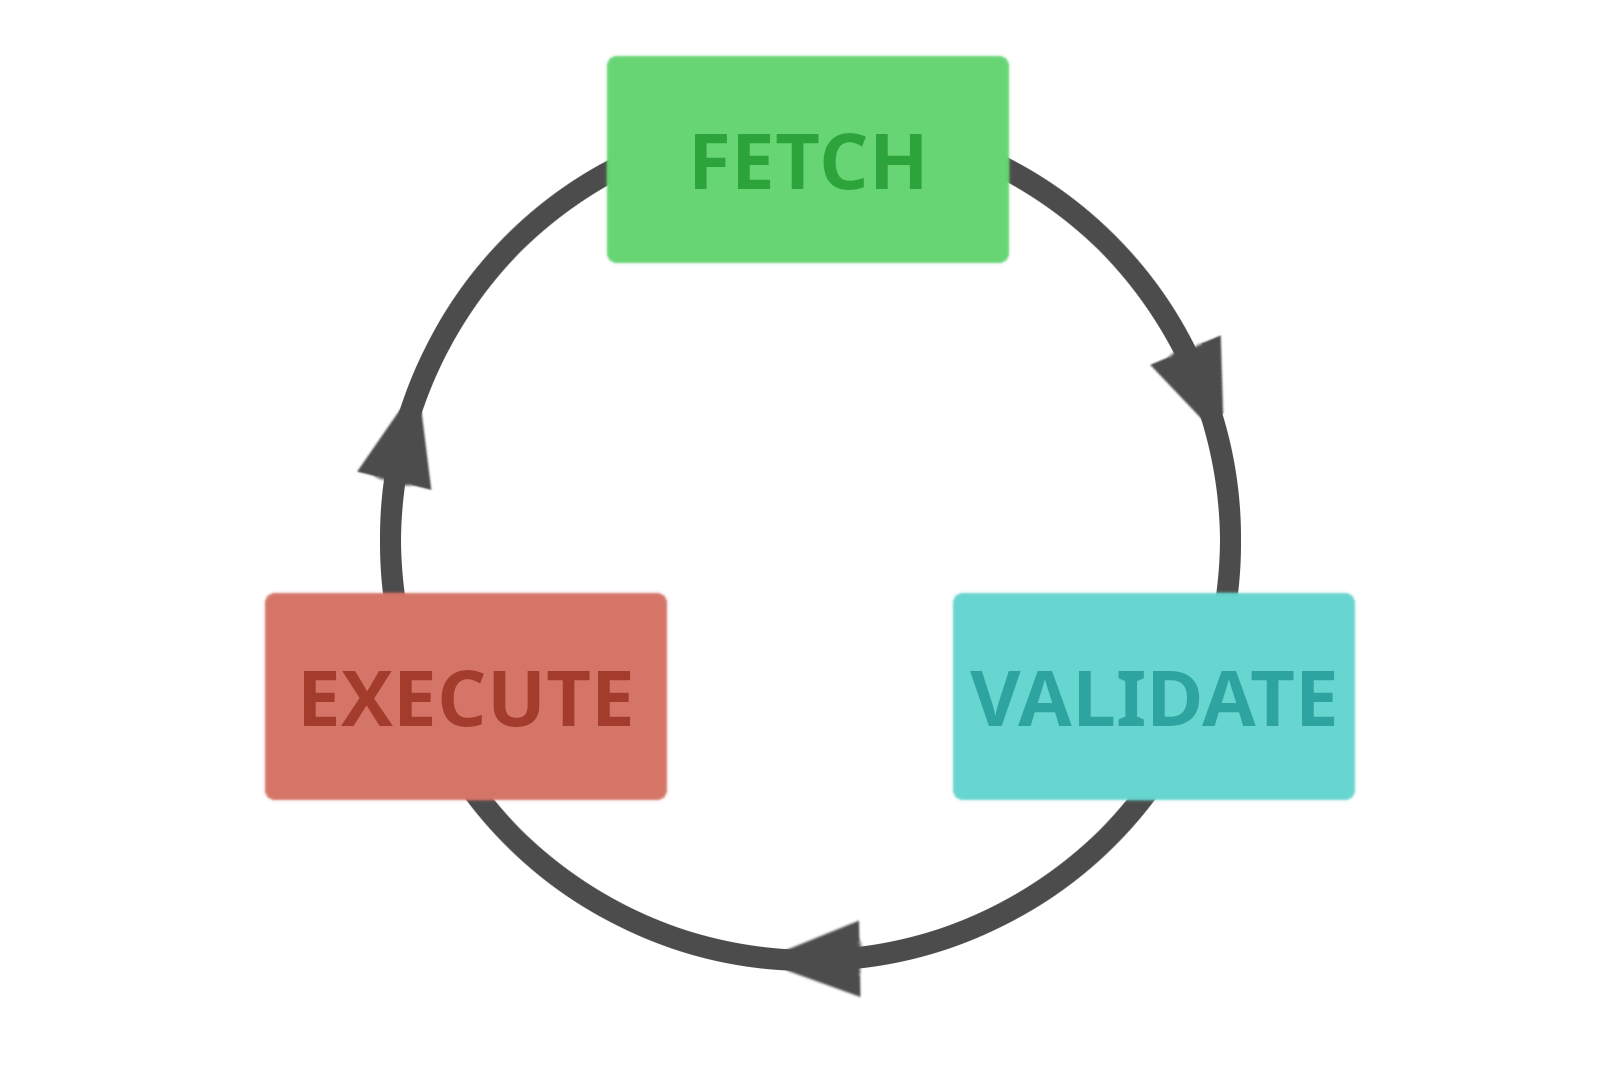
\includegraphics[scale=0.6]{resources/images/qhs-cycle.png}
    \caption{Zyklus der QHS Kompilierung (QHS-Zyklus)}
    \label{fig:qhs-cycle}
\end{figure}

\section{Fetch} \label{sec:qhs-fetch}
Die Aufgabe von \textit{Fetch} ist es die nächste Order, die verarbeitet werden soll, zu finden.
Der \textit{QHS-Zyklus} beginnt mit dem ersten Fetch. Dabei wird die erste Order aus der Inputdatei extrahiert. Bei jedem weiteren Fetch wird nun die nächste Order aus der Inputdatei geholt.
Eine Order weist wie erwähnt einen der drei Typen Identifier, Instruction oder LiteralCode auf.
Diese sind mit folgenden RegEx definiert. Whitespaces dienen als Trennung zwischen zwei Orders und werden ignoriert.

\begin{table}[h]
    \centering
    \caption{RegEx Definitionen der Order Typen}
    \vspace{3mm} % Adjust the height of the space between caption and tabular
    
    \begin{tabular}{ll}
    \multicolumn{1}{l|}{identifier}        & \textless{}identiferChar\textgreater{}*                           \\ \hline
    \multicolumn{1}{l|}{instruction}       & \# \textless{}identiferChar\textgreater{}*                        \\ \hline
    \multicolumn{1}{l|}{literalCode}       & ".*"                                                              \\
                                           &                                                                   \\
    \textless{}identiferChar\textgreater{} & = {[}\textasciicircum{}\# "\textless{}whitespace\textgreater{}{]} \\
    \textless{}whitespace\textgreater{}    & = SPACE | NEWLINE | TAB
    
    \end{tabular}
\end{table}

Im Vergleich zu traditionellen Compilern fällt auf, dass beim QHScompiler kaum zwischen Zeichen differenziert wird. Während die Lexical Analysis traditionell zwischen vielen verschiedenen Tokens unterscheidet,
sind für den QHScompiler alle Zeichen (mit Ausnahme von \# und " ) gleichbedeutend.

Bei einem Fetch kommt die nächste Order wie erwähnt von der Inputdatei.
Es ist jedoch möglich Orders voranzustellen. Diese Orders werden beim nächsten Fetch zuerst gefunden. Dies geschieht mithilfe des \textit{FetchStacks}, auf den Orders gelegt werden können.
Beim nächsten Fetch wird immer die oberste Order des FetchStacks geholt und daraufhin vom FetchStack enfernt.
Die Inputdatei befindet sich auf dem untersten Platz des FetchStacks und wird somit nur verwendet, wenn der Stack ansonsten komplett leer ist.
Eine Order kann während jedem der drei Schritte des Zyklus auf den FetchStack gelegt werden.
Während der Laufzeit des QHScompilers könnte der FetchStack folgendermassen aussehen:

\begin{figure}[h!]
    \centering
    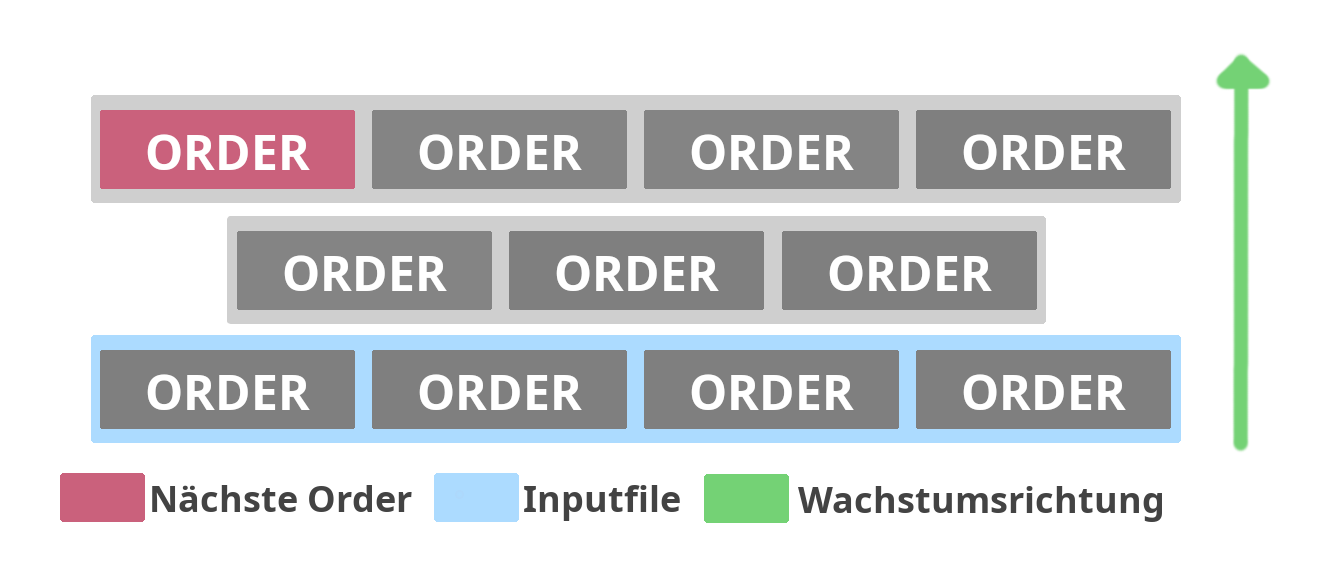
\includegraphics[scale=1.1]{resources/images/fetch-stack.png}
    \caption{Struktur des FetchStacks UPDATE}
    \label{fig:fetchstack}
\end{figure}

Die Hauptanwendung des FetchStacks wird im Abschnitt \ref{sec:qhs-execute} erklärt.
Die Kompilierung ist beendet, sobald keine Order mehr auf dem FetchStack vorhanden ist.

\section{Validate} \label{sec:qhs-Validate}
Nachdem die nächste Order durch Fetch gefunden wurde, wird diese Order an Validate weitergegeben. Während dem Validate Schritt kommt die \textit{OrderQueue} ins Spiel. Hierbei handelt es sich, wie der Name schon sagt, um eine Queue an Orders.
Die Aufgabe der OrderQueue ist das Speichern und spätere Zurückholen von Orders. Die OrderQueue kann mit Instructions, die im Abschnitt \ref{sec:qhs-execute} weiter ausgeführt werden, aktiviert und deaktiviert werden.
Wenn eine Order in den Validate Schritt gelangt und die OrderQueue aktiviert ist, wird diese Order der OrderQueue hinzugefügt. Der Execute Schritt wird danach übersprungen und der QHS-Zyklus beginnt von neuem bei Fetch.
Die Order wurde, ohne Execute erreicht zu haben, auf der OrderQueue gespeichert. Später ist es mit Instructions möglich diese Order von der OrderQueue zu entfernen und auszuführen.

Bestimmte Orders können jedoch orderQueue-proof, also immun gegen die OrderQueue, gemacht werden. Orders, die orderQueue-proof sind, werden an Execute weitergegeben, auch wenn die OrderQueue aktiv ist.
Dieses Prinzip ist zum Beispiel besonders bei der Instruction, die die OrderQueue wieder deaktiviert, wichtig. Da diese Instruction ansonsten nicht zu Execute gelänge und somit die OrderQueue nie deaktiviert würde.
Zu beachten ist, dass LiteralCode nicht orderQueue-proof sein kann.

MAYBE CODESTACK FIGURE

Ist die OrderQueue deaktiviert oder die Order orderQueue-proof, wird diese Order an den letzten Schritt Execute weitergegeben.

\section{Execute} \label{sec:qhs-execute}
Execute ist der letzte Schritt des QHS-Zyklus. Hier wird der tatsächliche Assembly Code generiert. Je nach Typ der Order (Identifier, Instruction oder LiteralCode) läuft Execute sehr unterschiedlich ab.

\subsection{Identifier}
Ein Identifier ist eine Zusammenfassung von mehreren Orders. Diese sind in einem \textit{Environment} definiert.
Hierbei handelt es sich um eine einfache Map, die einen Identifier mit einer Liste an Orders verknüpft.
In anderen Programmiersprachen werden Environments auch als Scope bezeichnet.
Wenn nun ein Identifier in den Execute Schritt kommt, werden die dazugehörigen Orders auf den FetchStack aus Abschnitt \ref{sec:qhs-fetch} gelegt.
Bei den nächsten Fetches werden nun zuerst die zum Identifier gehörenden Orders nacheinander abgebaut. Einfach ausgedeückt wird der Identifier im Inputfile mit seinen Orders ersetzt.

Die bereits erwähnten Environments sind dabei in einer Linked-List gespeichert. Somit können neue Environments zu dieser Liste hinzugefügt und von der Liste entfernt werden.
Das unterste Environment der Liste ist das älteste und das oberste Environment das neuste.
Ein neuer Identifier wird immer zum obersten Environment hinzugefügt. Definitionen des gleichen Identifiers in älteren Environments werden nicht überschrieben oder gelöscht.
Bei der Abfrage nach einem Identifier wird immer die neuste vorhandene Definition zurückgegeben. Ist keine vorhanden, wird ein Error ausgegeben.

\subsection{Instructions}
Instructions sind die komplexesten Orders für den Execute Schritt. Für jede Instruction ist im QHScompiler eine Funktion definiert, die ausgeführt wird, wenn diese Instruction in den Execute Schritt gelangt.
Diese Funktionen können Variablen im QHScompiler speichern, die OrderQueue aktivieren, Identifier definieren und vieles mehr. Instructions sind somit der Weg wie während der Kompilierung auf den QHScompiler einfluss genommen werden kann.
In der Tabelle \ref{tab:important_instructions} sind ein paar der wichtigsten Instructions aufgelistet:

\begin{table}[H]
    \centering
    \caption{Wichtige Instructions des QHScompilers}
    \label{tab:important_instructions}
    \vspace{3mm} % Adjust the height of the space between caption and tabular
    
    \begin{tabularx}{\textwidth}{l|X}
    \textbf{\#enterOrderQueue}      & Aktiviert die OrderQueue. \\ \hline
    \textbf{\#exitOrderQueue}       & Deaktiviert die OrderQueue. \\ \hline
    \textbf{\#assign}               & Die erste Order der OrderQueue muss ein Identifier sein. Der Rest der Orders auf der OrderQueue wird als Definition für diesen Identifier festgelegt. \\ \hline
    \textbf{\#assignToOne}          & Wie \#assign, jedoch wird nach dem Identifier nur eine weitere Order von der OrderQueue genommen und als Definition für den Identifier verwendet. \\ \hline
    \textbf{\#force}                & Die nächste Order wird nach Fetch sofort an Execute weitergegeben. Überspringt Validate und somit die OrderQueue. \\ \hline
    \textbf{\#lightForce}           & Ähnlich wird \#force, jedoch wird diese nur ausgeführt, wenn \textbf{explain this cuz they don't know OrderQueue depth} \\ \hline
    \textbf{\#orderEnqueue}         & Die nächste Order wird sofort der OrderQueue hinzugefügt, auch wenn diese Order orderQueue-proof wäre. Execute wird übersprungen. \\ \hline
    \textbf{\#orderFrontEnqueue}    & Ähnlich wie \#orderEnqueue. Die Order wird jedoch auf den obersten Platz der OrderQueue gesetzt. \\ \hline
    \textbf{\#deepFetch}            & Die nächste Order der Inputdatei wird oben auf den FetchStack gesetzt. Ermöglicht den Zugriff auf die Inputdatei innerhalb eines Identifiers. \\ \hline
    \textbf{\#queueFetch}           & Die oberste Order der OrderQueue wird oben auf den FetchStack gesetzt. \\ \hline 
    \textbf{\#pushEnv}              & Ein neues Environment wird der Environment Linked-List hinzugefügt. \\ \hline
    \textbf{\#popEnv}               & Das neuste Environment der Environment Linked-List wird gelöscht. \\ \hline
    \textbf{\#addLiterals}          & Die beiden obersten Orders auf der OrderQueue müssen LiteralCode sein. Diese werden als Zahl interpretiert und addiert. Sollten diese keine Zahl sein, wird ein Fehler gemeldet.        
    \end{tabularx}
\end{table}

Der QHScompiler umfässt \textbf{33} Instructions, wobei \textbf{5} dieser nur fürs Debugging des Compilers dienen.

\subsection{LiteralCode}
LiteralCode ist der Weg wie der QHScompiler Assembly Code generiert. Dieser ist sehr einfach. Wenn LiteralCode in den Execute Schritt gelangt, wird alles was zwischen den Satzzeichen steht in das Output-Dokument geschrieben.
Dies ist die einzige Möglichkeit für den QHScompiler Assembly Code zu generieren. Somit könnte nur durch das Ändern einzelner LiteralCode Orders die Output-Sprache des QHScompilers komplett geändert werden.


\section{Bringing it all together} \label{sec:qhs-bringing-it-together}
Und somit ist der QHScompiler komplett. Im Vergleich zu einem traditionellen Compiler wirkt der QHScompiler fast schon zu simpel. (... cuz function and vars and all of that hasn't even been mentioned) 
Dies hat einen einfachen Grund. Der QHScompiler ist zwar komplett, die dazugehörige Programmiersprache QHS jedoch noch lange nicht.
Grundsätzlich ist es möglich mit LiteralCode jedes Programm zu schreiben und zu kompilieren, jedoch handelt es sich dann nur um Assembly Code.
Doch der Aufbau des QHScompilers ermöglicht es mit Identifiern eine komplexere Programmiersprache zu definieren. Ein fester Bestandteil ein jedes Programms, das mit dem QHScompiler kompiliert werden soll, ist ein Stück Code,
das die jeweilige Programmiersprache definiert. Dieser Code wird im Kontext des QHScompilers \textit{Preamble} genannt. Theoretisch ist es möglich durch das Anpassen dieses Preambles, 
viele unterschiedliche Programmiersprachen mit dem QHScompiler zu kompilieren. In diesem Abschnitt wird behandelt wie sich die Sprache QHS, welche die Kriterien aus Abschnitt \ref{sec:Vergleichs_Kriterien} erfüllt,
für den QHScompiler definieren lässt.

\subsection{Abkürzungen}
Um die Leserlichkeit von QHS zu verbessern, werden ein paar Identifiers anstelle der umständlichen Instructions definiert.
Diese sind in der folgenden Tabelle \ref{tab:shortcuts} aufgeführt.

{
\begin{table}[H]
    \centering
    \caption{Identifiers als Abkürzung von Instruction}
    \vspace{3mm} % Adjust the height of the space between caption and tabular
    \label{tab:shortcuts}
    
    % select font of listing in first column (to be equivalent to listings)
    \begin{tabular}{>{\listingFont\selectfont}l|l}
    \textbf{{[}}                 & \#enterOrderQueue              \\ \hline
    \textbf{{]}}                 & \#exitOrderQueue               \\ \hline
    \textgreater{}\textgreater{} & \#assign                       \\ \hline
    \textbf{-\textgreater{}}     & \#assignToOne                  \\ \hline
    \textbf{!}                   & \#force                        \\ \hline
    \textbf{?!}                  & \#lightForce                   \\ \hline
    \textbf{\textbackslash{}n}   & Eine neue Zeile im Outputdatei
    \end{tabular}
\end{table}
}

Weiter wird innerhalb von Kommentaren Pseudo-Code verwendet, um den QHS Code verständlicher zu erklären. Kommentare können mehrere Zeilen umfassen und beginnen immer mit /* und enden mit */.
Der Kommentar /* X = "hello" \#pushEnv */ würde bedeuten, dass der Identifier X zu den Orders "hello" (LiteralCode) und \#pushEnv (Instruction) definiert wurde. 

Besonders bei längeren Identifier Definitionen wird zuerst der Identifier Name getrennt von den restlichen Orders der OrderQueue hinzugefügt.
Diese Separation dient der besseren Leserlichkeit und hat keinen Einfluss auf die Kompilierung des Codes.

\subsection{Identifier Parameter und Rückgabewert}
Mithilfe der \#enterOrderQueue und \#exitOrderQueue Instructions kann innerhalb eines Identifiers die OrderQueue verwendet werden. Dies ermöglicht eine Art von Parametern und Rückgabewert für Identifier.
Parameter werden vor dem Aufruf eines Identifiers der OrderQueue hinzugefügt. Diese kann dann der Identifier verwenden. Genauso kann der Identifier am Ende Orders der OrderQueue hinzufügen und diese somit zurückgeben.

\begin{lstlisting}[language=QHS, caption=Verwendung von Parametern und Rückgabewert eines Identifiers]
[ foo ]
[
    #orderFrontEnqueue param1 ->    /* param1 = erstes Argument */
    #orderFrontEnqueue param2 ->    /* param2 = zweites Argument */

    param1 " : " param2 \n          /* param1 + " : " + param2 + "\n" */

    [ "return" ]                    /* "return" wird der OrderQueue hinzugefügt */
] >>

[ "1" "2" ]                         /* 2 Argumente werden der OrderQueue hinzugefügt */
foo                                 /* foo wird ausgeführt */
#queueFetch                         /* Die zurückgegebene Order wird von der OrderQueue
                                    geholt und ausgeführt */


%\noindent\hrulefill Output\noindent\hrulefill%
1 : 2
return
\end{lstlisting}


\subsection{Variablen} \label{sec:qhs-vars}
Die Umsetzung von Variablen in QHS ist einfach. Zuerst soll der Assembly Code für das Abziehen der Grösse der Variable vom Stack-Pointer hinzugefügt werden.
Dann wird für die Variable ein Identifier definiert, der zur Position der Variable auf dem Stack zeigt.
Mit LiteralCode lässt sich dies wie folgt in QHS ausdrücken:

\begin{lstlisting}[language=QHS, caption=Definition einer Variable mit LiteralCode]
"sub rsp, 4" \n
[ a "[rbp-4]" ] >>      /* a = "[rbp-4]" */

"add " a ", 5"

%\noindent\hrulefill Output\noindent\hrulefill%
sub rsp, 4
add [rbp-4], 5
\end{lstlisting}

Jedoch braucht man für diese Implementation immer noch viel LiteralCode und Assembly Kenntnisse. Um die Definition von Variablen einfacher zu gestallten, lässt sich zum Beispiel ein \textit{var} Identifier definieren.
Dieser var Identifier nimmt die Grösse der Variable als Argument über die OrderQueue an. Um die in vielen Programmiersprachen geläufige Syntax der Definition einer Variable beizubehalten,
wird der Name der Variable mit der \#deepFetch Instruction beschafft.

\begin{lstlisting}[language=QHS, caption=Definition einer Variable mit \textit{var} Identifier]
[ var ]
[
    #orderFrontEnqueue size ->          /* size = argument1 */
    [ name ?! #deepFetch ] >>           /* name = Was nach dem var Identifier folgt */

    "sub rsp, " size \n

    [ ?! name "[rbp-4]" ] >>            /* var = "[rbp-4]" */
] >> 

[ "4" ] var a 

"add " a ", 5"
    
%\noindent\hrulefill Output\noindent\hrulefill%
sub 4
add [rbp-4], 5
\end{lstlisting}

Momentan erhält jede Variable jedoch noch die Addresse rbp-4, weswegen sich die Variablen gegenseitig überschreiben würden. Der momentane rbp-Offset muss also gespeichert und erhöht werden.
Dafür wird bereits am Anfang des Programms ein Identifier rbpOffset als 0 definiert. Mit der \#addToIdentifier Instruction, lässt sich nun rbpOffset erhöhen. Dies kann folgendermassen aussehen:

\begin{minipage}{\linewidth}
\begin{lstlisting}[language=QHS, caption=Definition einer Variable mit rbpOffset]
[ rbpOffset "0" ] >>                    /* rbpOffset = "0" */

[ var ]
[
    #orderFrontEnqueue size ->          /* size = argument1 */
    [ name ?! #deepFetch ] >>           /* name = Was nach dem var Identifier folgt */

    "sub rsp, " size \n

    [ rbpOffset ?! size ] #addToIdentifier      /* rbpOffset += size */

    [ ?! name "[rbp-" ?! rbpOffset "]" ] >>     /* var = "[rbp-OFFSET]" */
] >> 

[ "4" ] var a 
[ "8" ] var b 

"add " a ", 5"
"sub " b ", 10"
    
%\noindent\hrulefill Output\noindent\hrulefill%
sub rsp, 4
sub rsp, 8
add [rbp-4], 5
sub [rbp-12], 10
\end{lstlisting}
\end{minipage}

Zuletzt lässt sich das umständliche Hinzufügen der Grösse der Variable sowie der \textit{var} Identifier unter einem neuen Identifier zusammenfassen. Dies ist passenderweise die bekannte Bezeichnung für den Typen der Variable.

\begin{lstlisting}[language=QHS, caption=Definition einer Variable mit \textit{int} Identifier]
(...)

[ int ] 
[
    [ "4" ] var
] >>
    
int a 
int b 
    
"add " a ", 5"
"sub " b ", 10"
        
%\noindent\hrulefill Output\noindent\hrulefill%
sub rsp, 4
sub rsp, 8
add [rbp-4], 5
sub [rbp-12], 10
\end{lstlisting}

Nun sieht die Definition einer Variable genau so aus, wie es in anderen Programmiersprachen gebräuchlich ist.

\subsection{Funktionen} \label{sec:qhs-funcs}
Funktionen sind im Vergleich zu Variablen komplizierter. Nachfolgend sollen zwei der Probleme von Funktionsdefinitionen behandelt werden.

Anhand einer Funktionsdefinition, wie sie zum Schluss aussehen sollte, will ich die beiden Probleme erläutern:


\begin{lstlisting}[language=C, label=eg:qhs-function_goal, caption=Ziel für die Definition einer Funktion in QHS]
int foo ( int param1 , int param2 )
{
    (...)
}
\end{lstlisting}

Hier lässt sich bereits das erstes Problem feststellen. Im vorherigen Abschnitt \ref{sec:qhs-vars} wurde der \textit{int} Identifier für die Definition einer Variable verwendet. 
Das int in der Auflistung \ref{eg:qhs-function_goal} würde vom QHScompiler also als Definition für eine Variable verstanden werden. Der Unterschied zwischen Variable und Funktionsdefinition besteht hierbei in den Klammern,
die auf den Namen folgen. Der QHScompiler müsste also beim \textit{int} Identifier nach vorne schauen, ob sich eine Klammer nach dem Namen befindet, und folglich eine Variable oder Funktionsdefinition ausführen.
Dieses Vorgehen ist jedoch aufgrund des einfachen Designs des QHScompilers nicht möglich. Er kann bloss Orders ausführen, nicht jedoch überprüfen, ob eine Order vorhanden ist. Glücklicherweise lässt sich dieses erste Problem lösen,
ohne eine Änderung am QHScompiler vorzunehmen. Die Lösung basiert darauf, beim \textit{int} Identifier sowohl eine Variable als auch eine Funktionsdefinition vorzubereiten, aber keine der beiden bereits auszuführen.
Weiter wird eine Klammer als Identifier für eine Funktionsdefinition gesetzt, sowie ein Semikolon für die Definition einer Variable. Befindet sich nach dem Namen eine Klammer, wird eine Funktionsdefinition ausgeführt.
Ist dort aber ein Semikolon wird eine Variable definiert. Dieses Konzept wird im weiteren als \textit{DelayedExecute} bezeichnet. Das Ganze sieht danach wie folgt aus:

%minipage keeps the listing from splitting onto multiple pages
\begin{minipage}{\linewidth}
\begin{lstlisting}[language=QHS, caption=Implementation eines DelayedExecute für Definitionen]
[ function ]
[
    #orderFrontEnqueue returnSize ->        /* size = argument1 */
    #orderFrontEnqueue name ->              /* name = argument2 */

    [ ?! name ] #orderToLiteral ":" \n      /* "foo:" */
] >>

[ definition ]
[
    #orderFrontEnqueue size ->          /* size = argument1 */
    [ name ?! #deepFetch ] >>           /* name = Was nach dem var Identifier folgt */

    [ ; ]
    [
        [ #orderEnqueue ! size #orderEnqueue ! name ] var 
    ] >>
    /* ; = [ size name ] var */

    [ ( ]
    [
        [ #orderEnqueue ! size #orderEnqueue ! name ] function 
    ] >>
    /* ( = [ size name ] function */

] >>

[ int ]
[
    [ "4" ] definition
] >>
\end{lstlisting}
\end{minipage}


Das zweite Problem sind die Parameter eine Funktionsdefinition. Diese sehen genau gleich aus wie die Definition einer Variable, sollten jedoch vom QHScompiler anders ausgeführt werden.
Erstens sollte bei einer Parameterdefinition nicht der LiteralCode zur Subtraktion vom rsp hinzugefügt werden. Zweitens verwendet eine Parameterdefinition einen anderen rbp-Offset.
Die Lösung liegt im Umdefinieren des \textit{definition} Identifiers. Dieser ist momentan für die Definition von Variablen und Funktionen verantwortlich.
Bei der Anfangsklammer der Funktionsdefinition wird der \textit{definition} Identifier neu definiert, sodass er eine Parameterdefinition ausführt. Die vorherige Definition geht dank der \#pushEnv Instruction nicht verloren.
Bei der schliessenden Klammer wird \#popEnv durchgeführt, und der \textit{definition} Identifier ist wieder für Variablen und Funktionen zuständig. Diese Lösung wird im folgenden \textit{TempAssign} genannt.
Dies lässt sich in QHS wie folgt umsetzen:

\begin{minipage}{\linewidth}
\begin{lstlisting}[language=QHS, caption=Implementation eines TempAssigns für Parameter Definitionen]
[ function ]
[
    #pushEnv

    #orderFrontEnqueue returnSize ->        /* size = argument1 */
    #orderFrontEnqueue name ->              /* name = argument2 */

    [ ?! name ] #orderToLiteral ":" \n      /* "foo:" */

    [ definition paramDefinition ]          /* definition = paramDefinition */

    #popEnv             /* Umdefinition von definition wird vergessen */
] >>
\end{lstlisting}
\end{minipage}

Der Identifier \textit{paramDefinition} ist gleich wie der \textit{var} Identifier aus Abschnitt \ref{sec:qhs-vars}. Jedoch wird anstelle von \textit{rbpOffset} ein neuer \textit{paramOffset} Identifier verwendet.

Nun fehlt nur noch etwas an der Funktionsdefinition, der Funktionsbody. Dieser ist vergleichsweise einfach. Die beiden geschwungenen Klammern werden zu einem leeren Identifier definiert und somit ignoriert.
Der gesamte Code innerhalb des Body wird ganz normal vom QHScompiler ausgeführt und an die Outputdatei angehängt. Das Endresultat sieht wie folgt aus:

\begin{lstlisting}[language=QHS, caption=Finale Definition einer Funktion in QHS]
int foo ( int param1 , int param2 )
{
    "add " param1 ", " param2
}

%\noindent\hrulefill Output\noindent\hrulefill%
foo:
add [rbp+16], [rbp+20]
\end{lstlisting}

Mit von DelayedExecute und TempAssign lässt sich also syntaktisch komplexen Code problemlos in QHS definieren und ausführen.

QHS weist noch viele weitere Identifier, die einen C-like Syntax ermöglichen, auf.
Diese Identifier werden hier jedoch nicht weiter betrachtet, da diese einem ähnlichen Prinzip wie die beschriebenen Definitionen von Variablen und Funktionen folgen. 


    






